

\section{Magnetisation renormalisation methods}
\label{sec:magn-renorm-meth}

We compare renormalisation after every step with the methods used to achieve constant $\abs{\mv}$ in \nmag and \magpar.

We use BDF2 because TR is equivalent to IMR for the undamped ODE problem...

(could do TR as well? But too many graphs/lines probably)


\subsection{The self-correcting LLG}
\label{sec:self-correcting-llg-results}

\begin{figure}
  \centering
  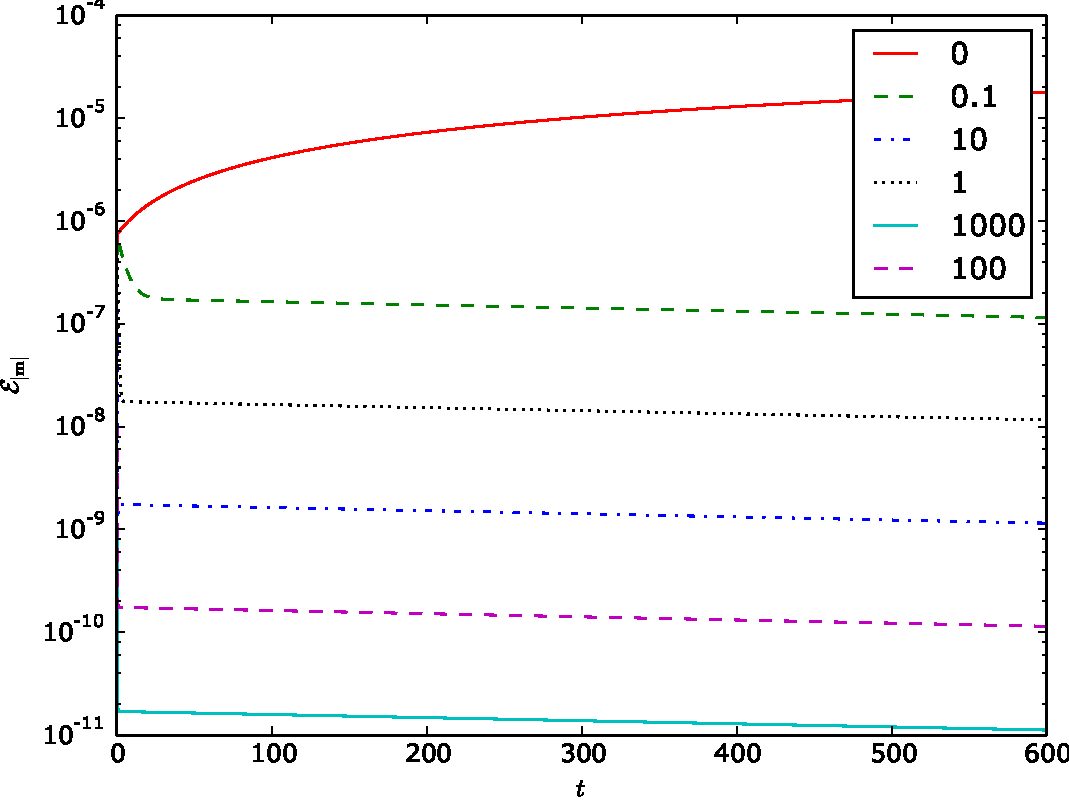
\includegraphics[width=0.8\textwidth]{plots//self_correcting_ode/0-mlengtherrormaxesvstimes.pdf}
  \caption{
    Error in magnetisation length against time for the ODE self-correcting LLG problem with
    $\dampc = 0$
    . Caption indicates the values of $\scc$.
  }
\end{figure}

\begin{figure}
  \centering
  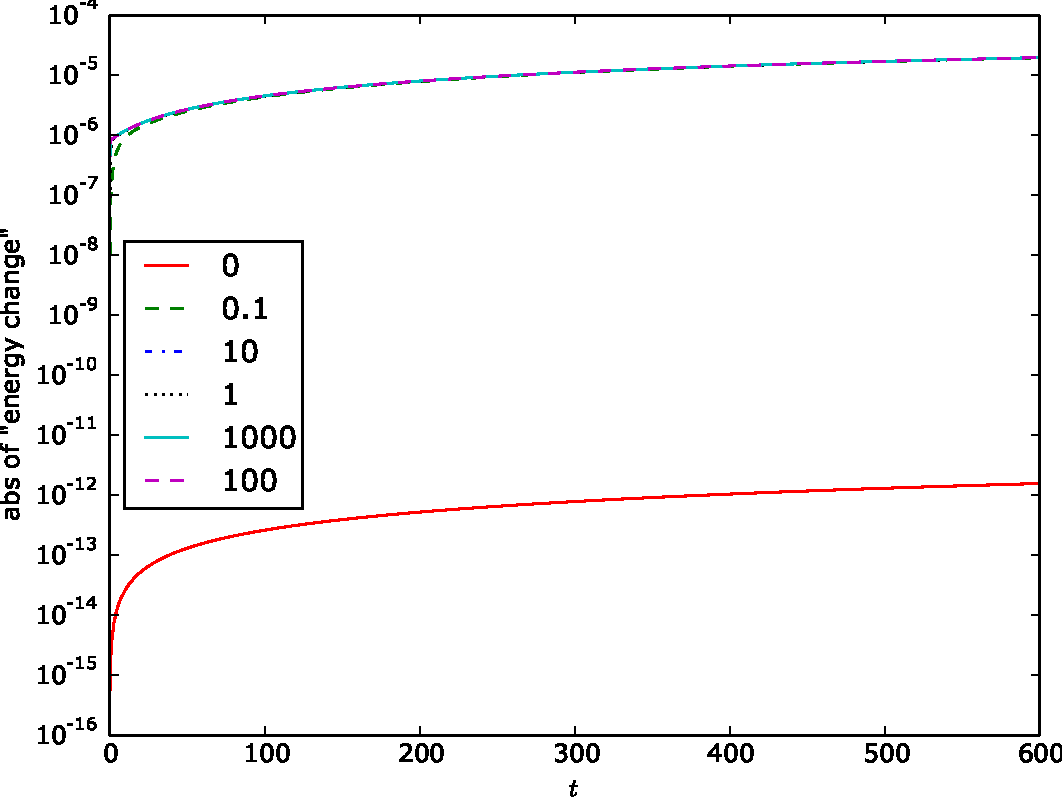
\includegraphics[width=0.8\textwidth]{plots//self_correcting_ode/0-absofenergychangevstimes.pdf}
  \caption{
    Error in energy against time for the ODE self-correcting LLG problem with
    $\dampc = 0$
    . Caption indicates the values of $\scc$.
  }
\end{figure}


\begin{figure}
  \centering
  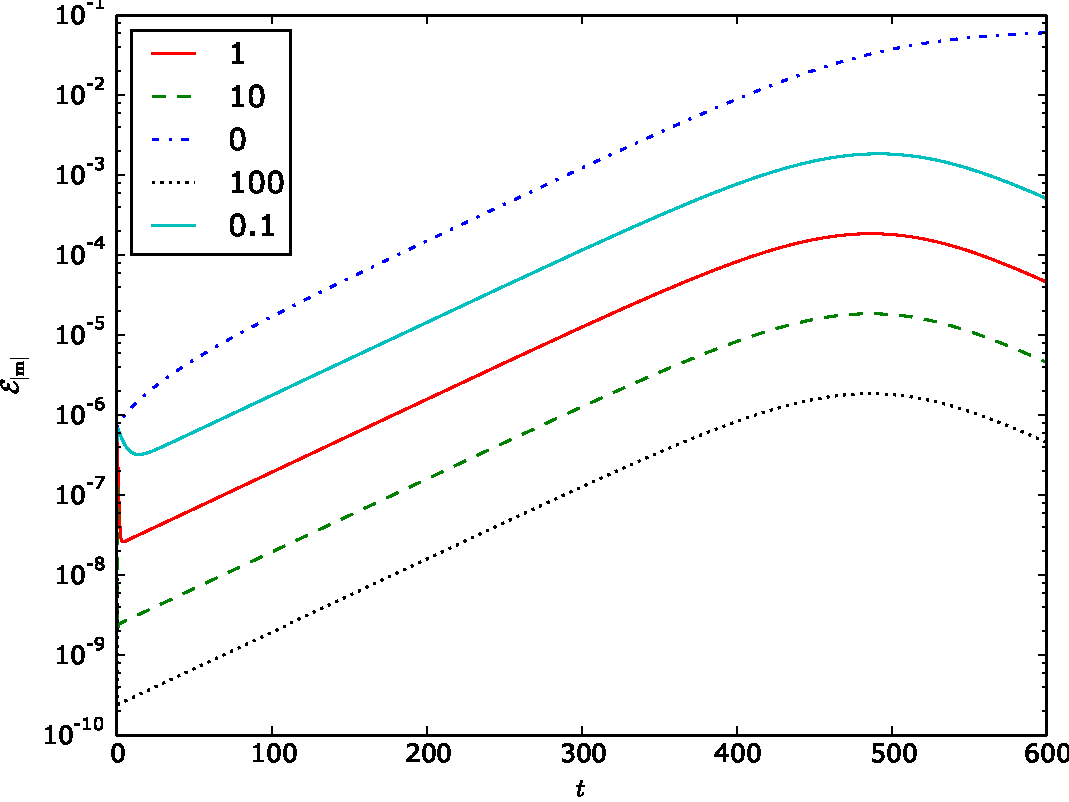
\includegraphics[width=0.8\textwidth]{plots//self_correcting_ode/001-mlengtherrormaxesvstimes.pdf}
  \caption{
    Error in magnetisation length against time for the ODE self-correcting LLG problem with
    $\dampc = 0.01$
    . Caption indicates the values of $\scc$.
  }
\end{figure}


Newton iterations vs beta? Also show IMR iters?

convergence plot


\subsection{Renormalisation after a tolerance}
\label{sec:renorm-after-toler}

Mag length errors vs time w/ varying tol, both dampings.

Energy errors

convergence

\subsection{Conclusions}

Self correcting LLG is always worse in controlling GI errors than renorm after each step: energy errors the same, m errors much larger.
It also takes additional newton step(s) (typically one more step is needed, increasing the computational time for the simulation by a factor of $\sim 3/2$).
Effect on convergence? ??ds
As such there appears to be no reason to use the self-correcting LLG over renormalisation after each step.


Renormalisation after a tolerance allows larger errors in $\abs{\mv}$ than renorm after each step (by definition).
It also introduces spurious oscillations in $\abs{\mv}$.
Effect on convergence ??ds
In terms of computational cost: checking whether renormalisation is needed has roughly the same cost as actually renormalising.
Hence there is no reason to prefer renormalisation after a tolerance.

%%% Local Variables:
%%% mode: latex
%%% TeX-master: "main"
%%% End:
